% Name: Fractal plant
% Description: A branching plant grown by a Lindenmayer system with brackets, which save and restore the turtle's place so each branch splits off and returns.
% Tags: fractal plant, L-system, branching, recursion

\usetikzlibrary{lindenmayersystems}

\pgfdeclarelindenmayersystem{Fractal plant}{
  \rule{X -> F+[[X]-X]-F[-FX]+X}
  \rule{F -> FF}}

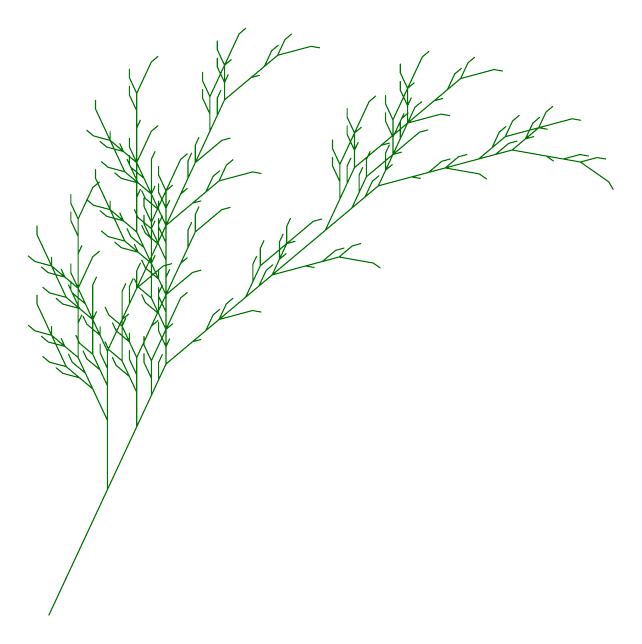
\begin{tikzpicture}
  \draw[green!45!black, line cap=round, rotate=65, lindenmayer system={Fractal plant, axiom=X, order=5, angle=25, step=1.1mm}] lindenmayer system;
\end{tikzpicture}
